%! TeX program = lualatex
\documentclass[a4paper]{article} 

% packages
\usepackage{microtype}      % Slightly tweak font spacing for aesthetics
\usepackage[english]{babel} % Language hyphenation and typographical rules
\usepackage[final, colorlinks = true, urlcolor = black, linkcolor = black]{hyperref} 
\usepackage{changepage}     % adjust margins on the fly

\usepackage{fontspec}
\setmainfont{EB Garamond}
\setmonofont[Scale=MatchLowercase]{Deja Vu Sans Mono}

\usepackage{minted}
\usemintedstyle{algol_nu}
\usepackage{xcolor}

\usepackage{pgfplots}
\pgfplotsset{width=\textwidth,compat=1.9}

\usepackage{caption}
\newenvironment{code}{\captionsetup{type=listing}}{}
\captionsetup[listing]{skip=0pt}
\setlength{\abovecaptionskip}{5pt}
\setlength{\belowcaptionskip}{5pt}

\usepackage[yyyymmdd]{datetime}
\renewcommand{\dateseparator}{--}

\usepackage{titlesec}
% \titleformat{\section}{\LARGE\bfseries}{}{}{}[\titlerule]
% \titleformat{\subsection}{\Large\bfseries}{}{0em}{}
% \titlespacing{\subsection}{0em}{-0.7em}{0em}
%
% \titleformat{\subsubsection}{\large\bfseries}{}{0em}{$\bullet$ }
% \titlespacing{\subsubsection}{1em}{-0.7em}{0em}

% margins
\addtolength{\hoffset}{-2.25cm}
\addtolength{\textwidth}{4.5cm}
\addtolength{\voffset}{-3.25cm}
\addtolength{\textheight}{5cm}
\setlength{\parskip}{0pt}
\setlength{\parindent}{0in}
% \setcounter{secnumdepth}{0}

\begin{document}
\hrule \medskip
\begin{minipage}{0.295\textwidth} 
    \raggedright
    \footnotesize 
    \begin{tabular}{@{}l l}
        Name: & Andrew Hayes \\
        Student ID: & 21321503 \\
        E-mail: & \href{mailto://a.hayes18@universityofgalway.ie}{\texttt{a.hayes18@universityofgalway.ie}} \\
    \end{tabular}
\end{minipage}
\begin{minipage}{0.4\textwidth} 
    \centering 
    \vspace{0.4em}
    \LARGE
    \textsc{ct414} \\ 
\end{minipage}
\begin{minipage}{0.295\textwidth} 
    \raggedleft
    \today
\end{minipage}
\medskip\hrule 
\begin{center}
    \normalsize
    Assignment 1: Java RMI
\end{center}
\hrule
\medskip

To run and test the code, I wrote a short shell script based off those provided in RMI Compute Server Example code provided on Canvas which compiles the code and launches three terminals: one running the \mintinline{shell}{rmiregistry}, one running the \mintinline{java}{ApplicationServer}, and one running the \mintinline{java}{ApplicationClient}.

\begin{code}
\inputminted[texcl, mathescape, linenos, breaklines, frame=single]{shell}{../code/src/run.sh}
\caption{\mintinline{shell}{run.sh}}
\end{code}

\begin{figure}[H]
    \centering
    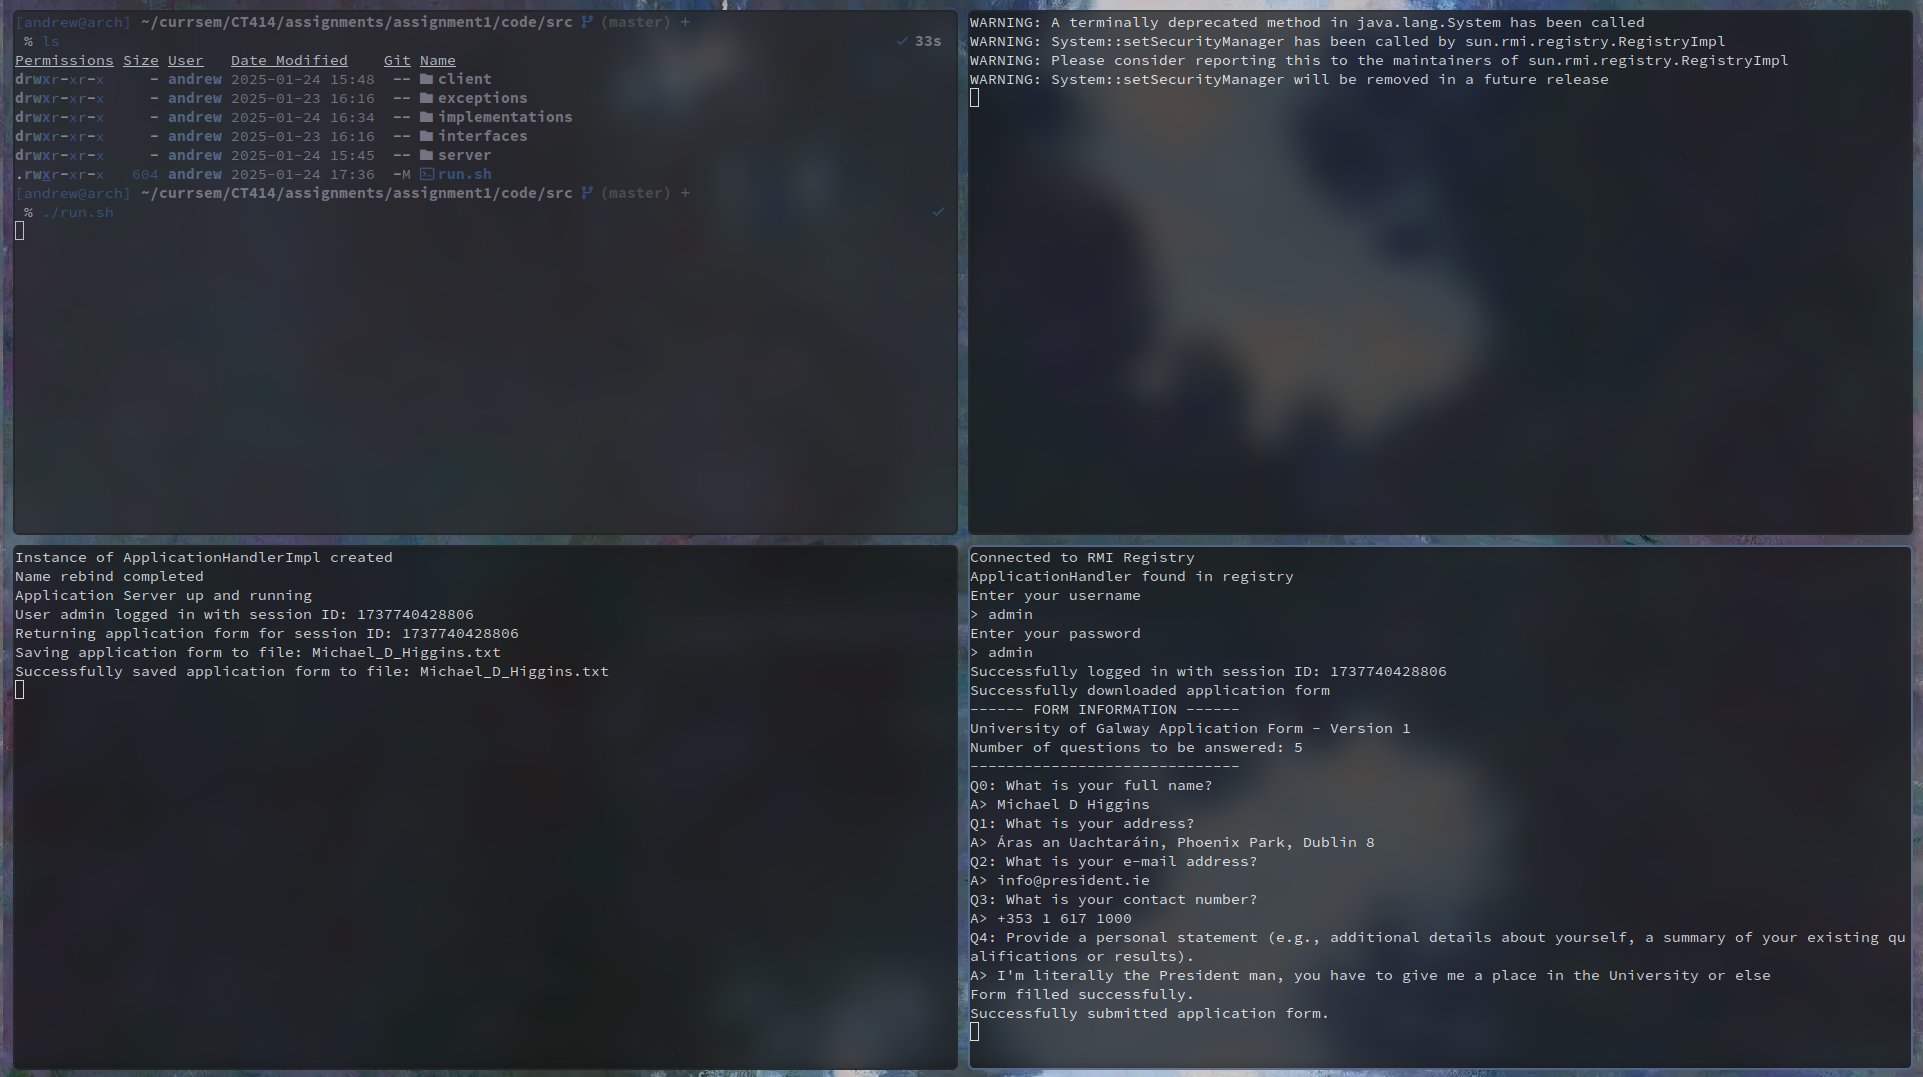
\includegraphics[width=\textwidth]{./images/screenshot.png}
    \caption{Screenshot of all four terminal windows. From left to right, top to bottom: the window running \mintinline{shell}{run.sh}, the window running the \mintinline{shell}{rmiregistry}, the window running the \mintinline{java}{ApplicationServer}, \& the window running the \mintinline{java}{ApplicationClient}}
\end{figure}

As can be seen in the \mintinline{java}{ApplicationClient} terminal window above, I tested the application by logging in with username \& password \verb|admin|, and filling in application details.
The details entered were saved into a file called \verb|Michael_D_Higgins.txt|, with the name of the file being the applicant's name with all whitespace replaced with underscores (to avoid any spaces-in-filename headaches).

\begin{figure}[H]
    \centering
    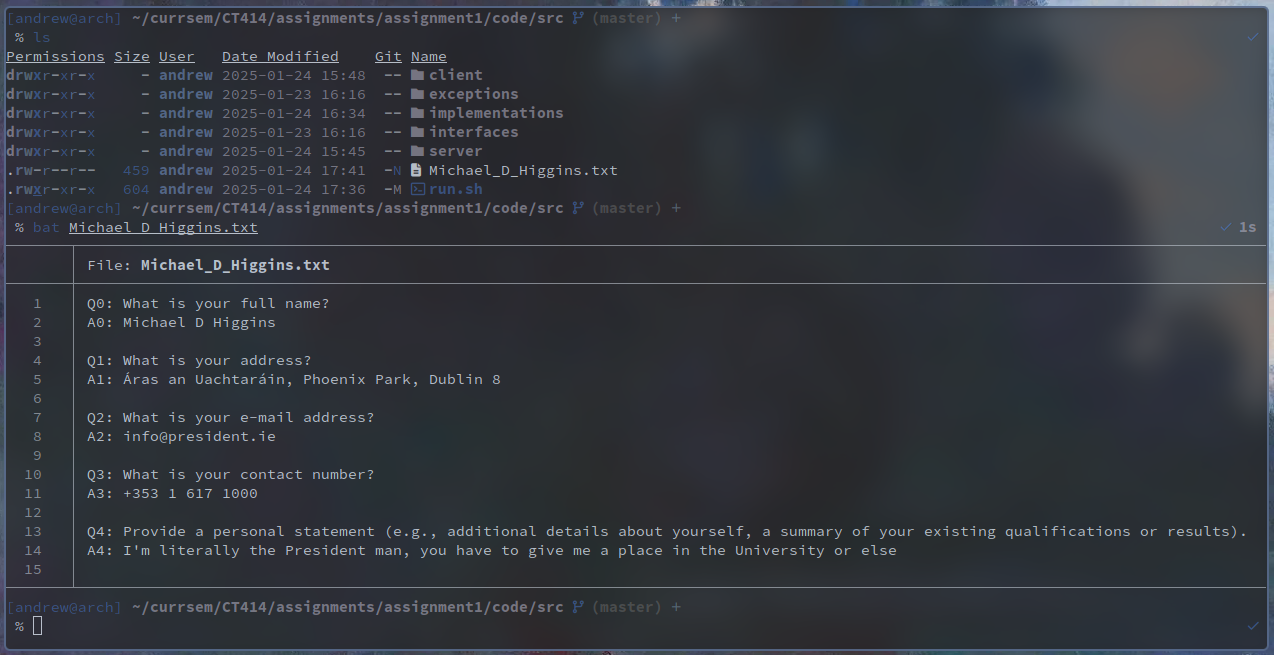
\includegraphics[width=\textwidth]{./images/michaeld.png}
    \caption{Contents of the saved application form file}
\end{figure}

The output file contained all the questions and answers from the application form, as expected.


\end{document}
